\chapter{Nambu String}

Now, we want to step over from field theory to string theory. In classical field theory, we got information about our fields in different points of spacetime. Here, we don't have points anymore but one-dimensional objects, called strings. At a given moment, one can move along the string that may change with time. So we need two coordinates, if we want to describe an event on the string. Nevertheless, it is important to keep the theory Lorentz invariant, so we have to work in four-dimensional spacetime. A very practical way is to take the two-dimensional surface and embed it into Minkowski spacetime:
\begin{figure}[H]
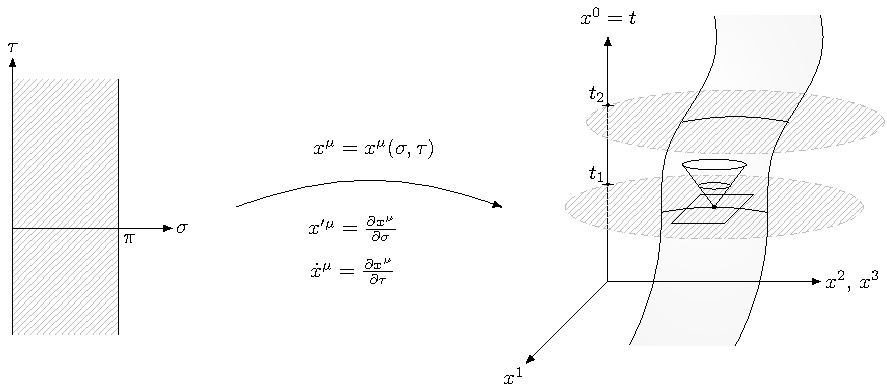
\includegraphics[width=\textwidth]{img/string.pdf}
\caption{Embedding of the Nambu string into Minkowski spacetime}
\label{fig:8}
\end{figure}
Here, $\sigma$ and $\tau$ denote the coordinates of the string at rest (the parametrization) and $x^{\mu}(\sigma, \tau)$ are the coordinates in spacetime. They depend on the inertial observer and can be transformed into each other by a Lorentz transformation. The sections of all embedded points with surfaces of constant time define the string at that moment. We choose $\sigma \in [0,\pi]$ because it is very practical for Fourier transformation which is often used in string theory, but we also could have chosen a different range. \\

Let us see now which conditions the embedding functions $x^{\mu}(\sigma, \tau)$ have to fulfill. First of all, it is very common to consider a closed string, that means identifying the endpoints 
\begin{align}
x^{\mu}(0, \tau) = x^{\mu}(\pi, \tau).
\end{align}
So the worldsheet of the string builds a kind of tube. \\

The second condition is that the string is not allowed to move faster than light ($\bar{v} \leq 1$). If a light signal is emitted on the string, the worldsheet is a cone with apex angle of $90^{\circ}$. The point of emission has to stay in the cone and is not allowed to exit (see Fig.~\ref{fig:8}). This corresponds to
\begin{align}
\dot{x}^2 = (\dot{x}^0)^2 - \dot{\bar{x}}^2 = \left( \frac{dx^0}{d\tau} \right)^2 - \left( \frac{d\bar{x}}{d\tau} \right)^2 \geq 1 - \left( \frac{d\bar{x}}{dx^0} \right)^2 \geq 0.
\end{align}

\pagebreak

And the last condition is that we want to have one time-like and one space-like vector. We found the time-like vector already which is just $\dot{x}^{\mu}$ because of the above condition. So we set the limitation 
\begin{align}
(x')^2 < 0,
\end{align}
and define $x'$ to be the space-like vector. The square should be understand as the inner product with Minkowski metric like in the condition above.


\section{Lagrangian}
What is the Lagrangian for such a string? 
We can try to rewrite the known Lagrangian of a relativistic point particle.
From special relativity, we know that the action of a point particle is 
\begin{align}
S = - m \int \sqrt{1 - \bar{v}^2} \ dt = - m \int \sqrt{(dt)^2 - (d\bar{x})^2} = - m \int \sqrt{dx_{\mu}dx^{\mu}} = - m \int ds. 
\end{align}
We see that the action corresponds to the "length" of the worldline of the particle, measured with Minkowski metric.
\begin{figure}[H]
\begin{center}
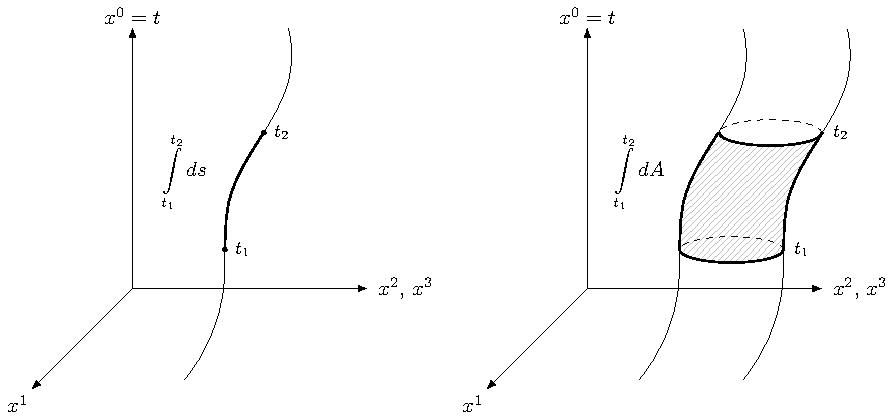
\includegraphics[width=\textwidth]{img/string_action.pdf}
\end{center}
\caption{Action of a relativistic point particle and a relativistic string}
\label{fig:9}
\end{figure}
Since now, we don't have a point which forms a worldline but a string which forms a "worldsuface", it is reasonable to take the area element instead of the line element and define
\begin{align}
S_{\text{str}} \equiv - \gamma \int dA,
\end{align}
where $\gamma$ is a proportionality constant. We will see later that this constant corresponds to the energy per unit length of the string.
But how to find the area element on the worldsheet of the string in Minkowski spacetime? \\

We will need a bit of differential geometry here. The area element on our flat parametrization would be given by $dA = d\sigma d\tau$. When we embed our surface into Minkowski spacetime, we have to consider the changing line elements (see Fig.~\ref{fig:10}):
\begin{align}
da^{\mu} &= \dot{x}^{\mu} d\tau \\
db^{\mu} &= x'^{\mu} d\sigma.
\end{align}
We could take this into account by using the generalized Jacobian determinant but we would like to show a more geometrical way.
\begin{figure}[H]
\begin{center}
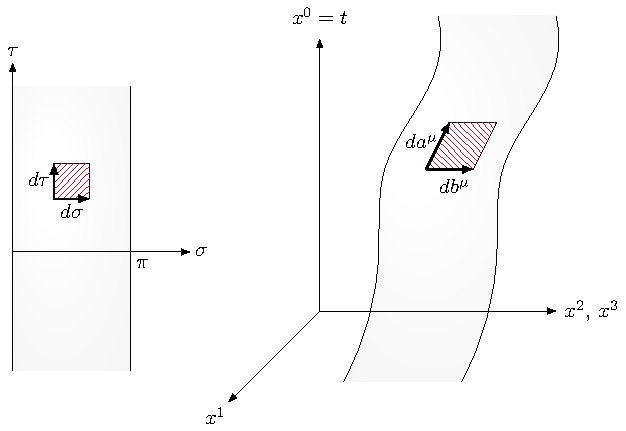
\includegraphics[scale=1.1]{img/string_area.pdf}
\end{center}
\caption{Finding the area element $dA$}
\label{fig:10}
\end{figure}
If an area is spanned by two vectors $\bar{a}, \bar{b}$ in three-dimensional euclidean space, the area is just
\begin{align}
A = |\bar{a} \times \bar{b}| = |\bar{a}| |\bar{b}| \sin(\measuredangle(\bar{a},\bar{b})) = |\bar{a}| |\bar{b}| \sqrt{1 - \left( \frac{\bar{a} \cdot \bar{b}}{|\bar{a}| |\bar{b}|} \right)^2} = \sqrt{|\bar{a}|^2 |\bar{b}|^2 - \left( \bar{a} \cdot \bar{b} \right)^2}.
\end{align}
But how to do it in four-dimensional Minkowski spacetime? If we want to know the area element of an embedded surface, we have to know the induced metric $g_{a b}$ on the surface. In our case, the area element turns out to be very similar to the three-dimensional case
\begin{align}
dA = \sqrt{|g|} \ d\sigma \wedge \tau = \sqrt{(\dot{x}x')^2 - \dot{x}^2(x')^2} \ d\sigma \wedge \tau,
\end{align}
as we will see later. Here $(\dot{x}x')$ denotes the inner product with our Minkowski metric and $x^{\mu}$ still depends on $\sigma$ and $\tau$. So the action for the Nambu string is
\begin{align}
S_{\text{str}} = - \gamma \int dA &= - \gamma \int \sqrt{(\dot{x}x')^2 - \dot{x}^2(x')^2} \ d\sigma d\tau \notag \\
&= - \gamma \displaystyle\int\limits_{\tau_1}^{\tau_2} d\tau \displaystyle\int\limits_{0}^{\pi} d\sigma \sqrt{(\dot{x}x')^2 - \dot{x}^2(x')^2}.
\end{align}


If we identify $\tau$ as the proper time, we can read off the Lagrangian for the Nambu string:
\begin{align}
L[x^{\mu}(\sigma), \dot{x}^{\mu}(\sigma)] = - \gamma \displaystyle\int\limits_{0}^{\pi} d\sigma \sqrt{(\dot{x}x')^2 - \dot{x}^2(x')^2}.
\end{align}




\section{Hamiltonian}

Now that we have the Lagrangian for the Nambu string, we can continue to find the Hamiltonian and see which constraints we get. In some sense, the description of string theory is similar to that of electrodynamics, we just take the coordinates $x^{\mu}$ instead of the fields $A_{\mu}$ and get
\begin{align}
q_i(t) \ \ \longrightarrow \ \ x^{\mu}(\sigma, \tau),
\end{align}
so the index $i$ is now given by $\mu$ and the position $\sigma$ on the string. The generalized momentum is therefore
\begin{align}
p_{\mu}(\sigma) = \frac{\delta L}{\delta \dot{x}^{\mu}(\sigma)}.
\end{align}
Let us calculate it for the Nambu string:
\begin{align}
p_{\mu}(\sigma) &= \frac{\delta L}{\delta \dot{x}^{\mu}(\sigma)} =  - \gamma \displaystyle\int\limits_{0}^{\pi} d\tilde{\sigma} \ \frac{2 (\dot{x}x') \frac{\delta(\dot{x}^{\nu}x'_{\nu})}{\delta \dot{x}^{\mu}(\sigma)} - (x')^2 \frac{\delta (\dot{x}^{\nu}\dot{x}_{\nu})}{\delta \dot{x}^{\mu}(\sigma)}}{2 \sqrt{(\dot{x}x')^2 - \dot{x}^2(x')^2}} \notag \\
&= - \gamma \displaystyle\int\limits_{0}^{\pi} d\tilde{\sigma} \ \frac{(\dot{x}x') \delta_{\mu}^{\nu} \delta(\sigma - \tilde{\sigma}) x'_{\nu} - (x')^2 \dot{x}_{\mu} \delta(\sigma - \tilde{\sigma})}{\sqrt{(\dot{x}x')^2 - \dot{x}^2(x')^2}} \notag \\
&= - \gamma \ \frac{(\dot{x}x') x'_{\mu} - (x')^2 \dot{x}_{\mu}}{\sqrt{(\dot{x}x')^2 - \dot{x}^2(x')^2}},
\end{align}
where the $x^{\mu}$ in the first and second line depend on $\tilde{\sigma}$ and in the last line on $\sigma$. It would be a difficult task to invert this equation and find $\dot{x}_{\mu}(p_{\mu})$ but fortunately we notice that
\begin{align}
px' \equiv p_{\mu}(\sigma) x'^{\mu}(\sigma) = - \gamma \ \frac{(\dot{x}x') (x')^2 - (x')^2 (\dot{x}x')}{\sqrt{(\dot{x}x')^2 - \dot{x}^2(x')^2}} = 0.
\end{align}

Moreover we have
\begin{align}
p^2 \equiv p_{\mu}(\sigma) p^{\mu}(\sigma) &= \gamma^2 \ \frac{(\dot{x}x')^2 (x')^2 - 2 (x')^2 (\dot{x}x')^2 + (x')^4 \dot{x}^2}{(\dot{x}x')^2 - \dot{x}^2(x')^2} \notag \\
&= - \gamma^2 \ \frac{(x')^2 \left[ (\dot{x}x')^2 - (x')^2 \dot{x}^2 \right]}{(\dot{x}x')^2 - \dot{x}^2(x')^2} \notag  \\
&= - \gamma^2 (x')^2.
\end{align}
So we get two primary constraints 
\begin{align}
\phi_1(\sigma) &= p(\sigma) x'(\sigma) = 0 \\
\phi_2(\sigma) &= p^2(\sigma) + \gamma^2 x'^2(\sigma) = 0.
\end{align}

These are already all constraints that we can find because in our case:
\begin{align}
\text{Number of constraints} = 4 - \text{rank} \left( \frac{\delta^2 L}{\delta\dot{x}^{\mu} \delta\dot{x}^{\nu}} \right).
\end{align}
One can show by explicit calculation that the rank of this matrix is two and that we only have two constraints but we won't do it here. \\

The next step is to find the Hamiltonian:
\begin{align}
H[x^{\mu}(\sigma), p^{\mu}(\sigma)] &\equiv \displaystyle\int\limits_{0}^{\pi} d\sigma \ \dot{x}_{\mu}(\sigma)p^{\mu}(\sigma) + \gamma \displaystyle\int\limits_{0}^{\pi} d\sigma \sqrt{(\dot{x}x')^2 - \dot{x}^2(x')^2} \notag \\
&= \displaystyle\int\limits_{0}^{\pi} d\sigma \left( - \gamma \frac{(\dot{x}x')^2 - (x')^2 \dot{x}^2}{\sqrt{(\dot{x}x')^2 - \dot{x}^2(x')^2}} + \gamma \sqrt{(\dot{x}x')^2 - \dot{x}^2(x')^2} \right) \notag \\
&= 0.
\end{align}
We notice that it is zero and in fact, we didn't even had to calculate the Hamiltonian because we know from theorem~\ref{Theorem} that 
\begin{equation}
\text{if} \ \ \ L[x^{\mu}(\sigma), \lambda \dot{x}^{\mu}(\sigma)] = \lambda L[x^{\mu}(\sigma), \dot{x}^{\mu}(\sigma)] \ \ \ \ \Longrightarrow \ \ \ \ H[x^{\mu}(\sigma), p^{\mu}(\sigma)] = 0.
\end{equation}

The total Hamiltonian is therefore
\begin{align}
H_T[x^{\mu}(\sigma), p^{\mu}(\sigma)] = \displaystyle\int\limits_{0}^{\pi} d\sigma \Bigg( u_1(\sigma)\underbrace{(p(\sigma)x'(\sigma))}_{=\phi_1(\sigma)} + u_2(\sigma) \underbrace{(p^2(\sigma) + \gamma^2 x'^2(\sigma))}_{=\phi_2(\sigma)}  \Bigg).
\end{align}

Are these constraints conserved at every moment or do we have secondary constraints? \\
We get the equation of motion by
\begin{align}
\dot{g} = \left \{ g,H_T \right \} = \displaystyle\int\limits_{0}^{\pi} d\sigma \left( u_1(\sigma) \left \{ g,\phi_1(\sigma) \right \}  + u_2(\sigma) \left \{ g,\phi_2(\sigma) \right \} \right),
\end{align}

where
\begin{align}
\left \{ f,g \right \} \equiv \displaystyle\int\limits_{0}^{\pi} d\sigma \left( \frac{\delta f}{\delta x^{\mu}(\sigma)} \frac{\delta g}{\delta p_{\mu}(\sigma)} - \frac{\delta g}{\delta x^{\mu}(\sigma)} \frac{\delta f}{\delta p_{\mu}(\sigma)} \right).
\end{align}


We have to check whether
\begin{align}
0 &\overset{?}{=} \dot{\phi}_1(\tilde{\sigma}) = \displaystyle\int\limits_{0}^{\pi} d\sigma \left( u_1(\sigma) \left \{ \phi_1(\tilde{\sigma}),\phi_1(\sigma) \right \}  + u_2(\sigma) \left \{ \phi_1(\tilde{\sigma}),\phi_2(\sigma) \right \} \right) \\
0 &\overset{?}{=} \dot{\phi}_2(\tilde{\sigma}) = \displaystyle\int\limits_{0}^{\pi} d\sigma \left( u_1(\sigma) \left \{ \phi_2(\tilde{\sigma}),\phi_1(\sigma) \right \}  + u_2(\sigma) \left \{ \phi_2(\tilde{\sigma}),\phi_2(\sigma) \right \} \right).
\end{align}

\pagebreak

Using the identity $\left \{ x^{\mu}(\sigma) , p_{\nu}(\tilde{\sigma}) \right \} = \delta_{\nu}^{\mu} \delta(\sigma - \tilde{\sigma})$ and calculating the poisson brackets accurately, one gets:
\begin{align}
\left \{ \phi_1(\tilde{\sigma}),\phi_1(\sigma) \right \} &=  (\phi_1(\sigma) + \phi_1(\tilde{\sigma})) \frac{\partial}{\partial \sigma}\delta(\sigma - \tilde{\sigma}) \\
\left \{ \phi_2(\tilde{\sigma}),\phi_2(\sigma) \right \} &= (\phi_1(\sigma) + \phi_1(\tilde{\sigma})) \frac{\partial}{\partial \sigma}\delta(\sigma - \tilde{\sigma}) \\
\left \{ \phi_1(\tilde{\sigma}),\phi_2(\sigma) \right \} &= (\phi_2(\sigma) + \phi_2(\tilde{\sigma})) \frac{\partial}{\partial \sigma}\delta(\sigma - \tilde{\sigma}).
\end{align}
So when we insert this in the above equations for $\dot{\phi}_1$ and $\dot{\phi}_2$, we see that they can be expressed by the constraints themself and therefore vanish on the constraint surface. \\
So these two constraints are first-class constraints and we get no secondary constraints, $u_1$ and $u_2$ stay arbitrary. \\


Since we have two arbitrary functions in our Hamiltonian, we have mathematical degrees of freedom or gauge freedom. The constraints are generators of gauge transformations. 

What transformations do they generate?
\begin{align}
\delta g = \varepsilon_m \left\{ g,\phi_m \right\} \ \ \ \Longrightarrow \ \ \ \delta g = \displaystyle\int\limits_{0}^{\pi} d\tilde{\sigma} \ \varepsilon(\tilde{\sigma}) \left\{ g,\phi(\tilde{\sigma}) \right\}.
\end{align}

Let's see which transformations $\phi_1$ generates for the coordinates $x^{\mu}$:
\begin{align}
\delta x^{\mu}(\sigma) &=  \displaystyle\int\limits_{0}^{\pi} d\tilde{\sigma} \ \varepsilon_1(\tilde{\sigma}) \left \{ x^{\mu}(\sigma),(p_{\nu}(\tilde{\sigma}) x'^{\nu}(\tilde{\sigma}) ) \right \} \notag \\
&=  \displaystyle\int\limits_{0}^{\pi} d\tilde{\sigma} \ \varepsilon_1(\tilde{\sigma}) x'^{\nu}(\tilde{\sigma}) \left \{ x^{\mu}(\sigma),p_{\nu}(\tilde{\sigma}) \right \} \notag \\
&= \varepsilon_1(\sigma) x'^{\mu}(\sigma) .
\end{align}
How to interpret this result? One can see that this is just the first order of the Taylor expansion of $x^{\mu}(\sigma + \varepsilon_1(\sigma))$:
\begin{align}
x^{\mu}(\sigma) \ \longrightarrow \ \tilde{x}^{\mu}(\sigma) = x^{\mu}(\sigma) + \varepsilon_1(\sigma) x'^{\mu}(\sigma) = x^{\mu}(\overbrace{\sigma + \varepsilon_1(\sigma)}^{= \tilde{\sigma}}).
\end{align}
So the transformation corresponds to a shift of the variable $\sigma$. That's why we have to impose the conditions
\begin{align}
\varepsilon_1(0) = \varepsilon_1(\pi) = 0,
\end{align}
to not exit the interval $[0,\pi]$:
\begin{align}
\tilde{\sigma}(0) &= 0 \\
\tilde{\sigma}(\pi) &= \pi.
\end{align}

It turns out that this transformation is a map from the string to itself. What changes effectively is the parametrization of the string but not the form of the string itself. \\
It's like we would reparametrize a path. Since we have many possible ways to choose a parametrization, this corresponds to a high degree of freedom. \\

For this moment, we don't want to concentrate on the possible gauge transformations. The other transformations can be found easily, analog to the above procedure. Rather, we want to consider a concrete gauge (a concrete value of the arbitrary functions) and see what dynamics follow from it. 


\section{Dynamics}

Let us choose the gauge:
\begin{align}
u_1(\sigma) &= 0 \\
u_2(\sigma) &= \frac{1}{2 \gamma} 
\end{align}

and calculate the Hamiltonian equations of motion for the coordinates:
\begin{align}\label{eq:78}
\dot{x}^{\mu}(\sigma) &= \left \{ x^{\mu}(\sigma), \frac{1}{2 \gamma} \displaystyle\int\limits_{0}^{\pi} d\tilde{\sigma} \left( p^2(\tilde{\sigma}) + \gamma^2 x'^2(\tilde{\sigma}) \right) \right \} \notag \\
&= \frac{1}{2 \gamma} \displaystyle\int\limits_{0}^{\pi} d\tilde{\sigma} \ 2 p^{\mu}(\tilde{\sigma}) \delta(\sigma - \tilde{\sigma}) \notag \\
&= \frac{p^{\mu}(\sigma)}{\gamma}
\end{align}

and for the momenta:
\begin{align}\label{eq:79}
\dot{p}^{\mu}(\sigma) &= \left \{ p^{\mu}(\sigma), \frac{1}{2 \gamma} \displaystyle\int\limits_{0}^{\pi} d\tilde{\sigma} \left( p^2(\tilde{\sigma}) + \gamma^2 x'^2(\tilde{\sigma}) \right) \right \} \notag \\
&= \frac{1}{2 \gamma} \displaystyle\int\limits_{0}^{\pi} d\tilde{\sigma} \ 2 \gamma^2 x'^{\nu}(\tilde{\sigma}) (- \delta^{\mu}_{\nu}) \frac{\partial}{\partial \tilde{\sigma}}\delta(\sigma - \tilde{\sigma}) \notag \\
&= \gamma x''^{\mu}(\sigma).
\end{align}

Inserting these results into our constraints $\phi_1(\sigma)$ and $\phi_2(\sigma)$, we get the conditions
\begin{align}
\dot{x}^2 + (x')^2 &= 0 \\
\dot{x} x' &= 0,
\end{align}
which means that $x'$ and $\dot{x}$ are orthogonal. That is why we call them \textit{orthonormal gauge}.

Moreover we can take the time-derivative of equation \eqref{eq:78} and insert equation \eqref{eq:79} to get the equation of motion
\begin{equation}\label{eq:eom}
\ddot{x}^{\mu}(\sigma, \tau) - x''^{\mu}(\sigma, \tau) = 0.
\end{equation}

This looks much like the equation $\partial_a \partial^a x^{\mu}(\sigma, \tau) = 0$, where $a = 1,2$ denote the derivative with respect to $\tau$ and $\sigma$, with signature $(+ -)$. That's why we would like to show the connection between $1+1$ gravity and the Nambu string before continuing with the dynamics. 

\begin{example}[$1+1$ Gravity] 
We want to illustrate the connection between the string and $1+1$ gravity, that is, one time-dimension and one space-dimension.
When we embed the string in Minkowski space, it can have curvature. What is the metric? 
The easiest way to find out the components of the metric is to look at the invariant line element  
\begin{align}
dx^{\mu} &= \dot{x}^{\mu} d\tau + x'^{\mu} d\sigma \\
ds^2 &= dx_{\mu}dx^{\mu} = \dot{x}^2 (d\tau)^2 + 2 \dot{x} x' d\tau d\sigma + (x')^2 (d\sigma)^2.
\end{align}
From here we can read off the metric since $ds^2 = g_{ab} \ dx^a dx^b$:
\begin{align}
g_{ab} = 
\begin{pmatrix}
    \dot{x}^2 & \dot{x} x' \\
    \dot{x} x' & (x')^2
  \end{pmatrix}
\end{align}
and with our orthonormal gauge conditions, we get
\begin{align}
g_{ab} = 
\begin{pmatrix}
    \dot{x}^2 & 0 \\
    0 & - \dot{x}^2
  \end{pmatrix}
= \dot{x}^2
\begin{pmatrix}
    1 & 0 \\
    0 & -1
  \end{pmatrix},
\end{align}
which is a conformally flat metric.
So we showed that the "worldsurface" of the string (like every two-dimensional Riemannian manifold) is conformally flat. This means that for every point on this surface, one can find a neighborhood that can be mapped to flat space by a conformal transformation (one that preserves orientation and angles locally). 
The signature is $(+ -)$ like expected.

Let's take a closer look at the action of the string again:
\begin{align}
S = - \gamma \int d\tau d\sigma \sqrt{(\dot{x} x')^2 - \dot{x}^2 (x')^2}.
\end{align}
We notice that the expression under the square root is exactly the negative of the determinant of the metric:
\begin{align}
g \equiv \mbox{det}(g_{ab}) = \dot{x}^2(x')^2 - (\dot{x}x')^2.
\end{align}
So we can write the action of the string as
\begin{align}
S = - \gamma \int d\tau d\sigma \sqrt{- g}
\end{align}
which is a kind of Einstein-Hilbert action for $1+1$ gravity, where $\gamma$ plays the role of a gravity constant. In $3+1$ gravity it takes the form 
\begin{align}
S = \frac{1}{2 \kappa} \int d^4 x \ \sqrt{- g} \ (R + \Lambda).
\end{align}
The string can be easily generalized to higher dimensions.
\end{example}


Let us continue with the dynamics of the Nambu string. We have still enough gauge freedom to set 
\begin{align}
t = x^0(\sigma, \tau) = \tau.
\end{align}
This choice is often used and leads to some simplifications in our dynamics. \\

It implies that
\begin{align}
\arraycolsep=1.4pt\def\arraystretch{1.5}
\begin{array}{ll}
\dot{x}^0 = \frac{\partial x^0}{\partial \tau} = \frac{\partial \tau}{\partial \tau} = 1 \ \ \ & \ \ \ x'^0 = 0 \\
\dot{\bar{x}} = \frac{\partial \bar{x}}{\partial \tau} = \frac{\partial \bar{x}}{\partial t} = \bar{v} \ \ \ & \ \ \ \bar{x}' = \frac{\partial \bar{x}}{\partial \sigma},
\end{array} 
\end{align}
which leads in connection with our constraints to
\begin{align}
\dot{x} x' = - (\dot{\bar{x}} \bar{x}') = 0
\end{align}
and 
\begin{align}
\dot{x}^2 + (x')^2 = (1 - \dot{\bar{x}}^2) - (\bar{x}')^2 = 0.
\end{align}
So we can replace our orthonormal gauge conditions by
\begin{align}
\dot{\bar{x}}^2 + (\bar{x}')^2 &= 1 \\
\dot{\bar{x}} \bar{x}' &= 0
\end{align}
and the equation of motion \eqref{eq:eom} turns to
\begin{align}
\ddot{\bar{x}}(\sigma, \tau) - \bar{x}''(\sigma, \tau) = 0.
\end{align}

So all our constraints and the equation of motion reduced to three dimensions.
Let's see how we can rewrite our Lagrangian:
\begin{align}
L &= - \gamma \displaystyle\int\limits_{0}^{\pi} d\sigma \sqrt{(\dot{x}x')^2 - \dot{x}^2(x')^2} \notag \\
&= - \gamma \displaystyle\int\limits_{0}^{\pi} d\sigma \ \sqrt{0 - (1 - \bar{v}^2) (- (\bar{x}')^2)} \notag \\
&= - \gamma \displaystyle\int\limits_{0}^{\pi} d\sigma \ \left| \bar{x}' \right|  \sqrt{1 - \bar{v}^2}.
\end{align}
It reduces also to three dimensions and looks quite similar to the Lagrangian of a relativistic point particle: $L = - m \sqrt{1 - \bar{v}^2}$. Let us define the length $S$ of the string:
\begin{align}
S = \displaystyle\int\limits_{0}^{\pi} d\sigma \ \left| \bar{x}' \right| = \displaystyle\int\limits_{0}^{S} ds.
\end{align} 

Then we get in analogy to the relativitic point particle:
\begin{align}
dm = \gamma \ ds \ \ \ \Longrightarrow \ \ \ \gamma = \frac{dm}{ds}.
\end{align}

We see that $\gamma$ corresponds to the mass/energy of the string per unit length as mentioned before. 